\documentclass[a5paper,twoside,openany]{book}
\usepackage[body={12cm,18cm}]{geometry}
\usepackage[a5,center,off]{crop}
\usepackage{titlesec}  % For customizing title formats
\usepackage{enumitem}
\usepackage{caption}
\pagestyle{plain}
\usepackage{graphicx}
\usepackage{wrapfig}
\usepackage{lipsum}
\graphicspath{ {./images/} }

\begin{document}


\setlength\parindent{0pt}

\titleformat{\chapter}[block]
  {\normalfont\huge\bfseries\centering} % Format for chapter title: huge font, bold
  {\thechapter} % Include the chapter number (e.g., "1")
  {1em} % Spacing between the chapter number and the title
  {} % Text before the chapter title (e.g., "Chapter 1 Title")

% Reducing title and section spacing  
\titlespacing*{\chapter} {0pt}{0ex}{0ex}

% Customizing the Table of Contents title
\renewcommand{\contentsname}{\small Sumario}
\renewcommand{\chaptername}{\small Capítulo}

% Title Page (optional)
\title{%
	Guía para aprender a reparar tus propios aparatos electrodomésticos y electrónicos\\
	\small (¡incluso si nunca has cogido un destornillador!)
	}

\author{%
	David M. \\
	\small Asociación \\ 
	"l'Ateliéphémère"  \\\\
	Traducción: RestartersVLC \\
	}

\maketitle

\tableofcontents
\newpage
 

% Example content
\chapter{Introducción}
\section{Presentación de L'ateliéphémère}

L'ateliéphémère es una asociación que ofrece talleres (así como cursos de formación sobre
sobre temas específicos) para ayudarte a aprender a reparar tus propios
equipos eléctricos y electrónicos, electrodomésticos, etc.\\

\textbf{\underline{¿Cómo funciona?}}

Alguien trae su electrodoméstico averiado, explica el problema y juntos intentamos repararlo.

Pero como siempre aprendemos mejor haciéndolo nosotros mismos, es la persona que ha traído
la persona que ha traído el aparato utilizará las herramientas disponibles in situ.
herramientas.

El objetivo de estos talleres es demostrarnos a nosotros mismos que somos capaces de
reparar muchas cosas uno mismo con muy pocos conocimientos y
conocimientos técnicos.

Todo el mundo es capaz de cambiar un fusible o poner un poco de aceite
¡en el lugar correcto!

Mis años de estudiante de electrónica no me enseñaron gran cosa que fuera útil para reparar un electrodoméstico, aparte de aprender a soldar y el vocabulario para investigar más fácilmente
después.

Esta guía te ayudará a sentirte más tranquilo cuando te enfrentes a un aparato que diagnosticar.
diagnosticar un aparato, sin tener que dedicar años de minucioso estudio
años de estudio o leer tediosamente libros de texto teóricos llenos de complicadas
¡complicadas fórmulas que no le ayudarán a arreglar su batidora!
Por supuesto, hay mucha información que no está ahí, pero hay enlaces a ella.
pero hay enlaces a una serie de foros al final de esta guía para ayudarte a
para ayudarte a encontrar más información.

Y si vives en la región Rhône-Alpes, estos talleres tienen lugar actualmente en
en Saint-Étienne, Grenoble y Lyon (y ocasionalmente más lejos), en centros sociales
en centros sociales, talleres comunitarios de ciclismo, bares comunitarios, etc.
La antigüedad de estos talleres nos permite llegar a personas que están
acostumbradas a los lugares donde se celebran los talleres y que, por tanto, se sienten cómodas
se sienten cómodos acudiendo sin demasiada aprensión.
No creo que baste con decir que un lugar está "abierto a todos".
para que vengan personas alejadas de ciertas redes (asociaciones, activistas, etc.).
¡que vengan!

\section{¿Por qué la realización de esta guía?}
En primer lugar, porque, que yo sepa, no existe ningún folleto o libro destinado a explicar de la forma más sencilla posible lo que hay que hacer.
explicar de la forma más sencilla posible lo que hay que saber para empezar a
a reparar la mayoría de los aparatos que nos rodean.

Existen libros sobre el tema, que pueden ayudar con las reparaciones, pero son demasiado técnicos  y, por tanto, de difícil acceso si no se tiene un mínimo de conocimientos en la materia.
El objetivo de esta guía es, por tanto, explicar los fundamentos esenciales de la electricidad
y, a continuación, los conocimientos y consejos que le permitirán iniciarse en la
reparación de un electrodoméstico.\\

He intentado mantener la sencillez y no explicar demasiadas cosas complejas que
que no te servirían de nada a la hora de reparar un electrodoméstico. Me he inspirado en casos
encontrados en mis talleres que reflejan las averías más comunes.
He enmarcado pasajes que he escrito a título informativo pero que no son
esenciales, por ejemplo las fórmulas, que rara vez se utilizan para Ce
diagnosticar una avería.
Por tanto, estos pasajes están ahí para los más curiosos.

Si no lees esta guía desde el principio, puede que no entiendas de qué estoy hablando.
entender de qué estoy hablando.
Como mínimo tendrás que leer el capítulo 2 sobre los fundamentos de la electricidad para poder
entender cómo probar cada uno de los componentes.\\

Esta guía no requiere ningún conocimiento ni habilidad. Está dirigida a cualquier persona que
personas que prefieren tomarse el tiempo de desmontar un aparato y ver
lo que ocurre en su interior, en lugar de tirarlo y comprar uno nuevo
y contribuir así al enorme despilfarro que se está produciendo.

\section{Sobre las consecuencias de la electrónica}

Para fabricar un chip de 2 gramos se necesitan 1,6 kg de energía fósil, es decir
600 veces su peso. Los ordenadores y todos los productos electrónicos y eléctricos
Los productos eléctricos plantean graves problemas al final de su vida útil.
Según Serge Latouche, en su libro "Bon pour la casse", actualmente
150 millones de ordenadores son transportados cada año a vertederos ilegales en el
vertederos ilegales del Tercer Mundo (500 barcos al mes salen hacia Nigeria y
Ghana).
En los documentales de Cosima Dannoritzer "Prêt à jeter" y "La tragedia", nos enteramos de que el 75\% de esta basura electrónica no se recicla.
La mayor parte es quemada por niños en enormes vertederos al aire libre para recuperar los
recuperar metales raros.

\textit{"Se calcula que, en el mundo desarrollado, alrededor del 75\% de estos residuos desaparece de los circuitos oficiales de reprocesamiento.
desaparece de los circuitos oficiales de reprocesamiento. Gran parte se exporta
ilegalmente, a vertederos clandestinos en África".
}
(http://greenfocusmag.com/ verite-e-waste-monde-afrique)

Por su composición, la electrónica es en cualquier caso muy complicada de reciclar.

Además de estos residuos, el \textbf{80\% de la electrónica mundial} se fabrica
en las fábricas de Foxconn en Shenzhen (subcontratistas de Apple, Acer, Blackberry
Dell, Google, Motorola, Toshiba, Asus....).

Esta "ciudad factoría" emplea a 1,4 millones de personas que trabajan 12 horas al día
día, 6 días a la semana por unos 150 euros.
En el primer semestre de 2010, se produjeron 14 suicidios en esta
fábrica. La principal respuesta a estos suicidios fue la instalación de redes "a prueba de suicidas" bajo el tejado de la planta.

(Leer en "La machine est ton seigneur et ton maître", publicado por Agone)

\section{Las 5 principales barreras para la reparación}
\begin{enumerate}
\item Falta de confianza en la propia capacidad de reparación.
Desde una edad temprana, las pantallas y los teclados están sustituyendo a las herramientas manuales.
\item El deseo de la industria de que los aparatos sean difíciles de
difíciles de desmontar: diseño "futurista", tornillos especiales o ausencia total de tornillos (moldeado, pegado, etc.).
\item La documentación técnica y los diagramas necesarios para comprender cómo funciona el
funcionamiento del equipo no se encuentran en ninguna parte.
\item Las piezas de repuesto ya no se fabrican o se fabrican a precios desalentadores.
precios desalentadores.
\item La publicidad que intenta convencernos de que necesitamos el nuevo modelo "más eficiente", "menos contaminante" (desperdiciar menos para contaminar menos...).
El resultado es lo que se conoce como "obsolescencia simbólica".
En 2002, más de 130 millones de teléfonos móviles en funcionamiento
se desecharon en Estados Unidos (Serge Latouche, "Bon pour la
Casse")
\end{enumerate}

\section{¿Y esto, se repara?}
En teoría, todo se puede reparar, pero en la práctica, sólo el 50\% de los aparatos (de todo tipo) salen de mis talleres en buen estado.
Principalmente por las barreras 2, 3 y 4 mencionadas anteriormente.
Además, con la llegada de los aparatos portátiles/desechables (teléfonos, tabletas, etc.)
que son cada vez más difíciles de reparar sin herramientas específicas, evolucionan demasiado rápido
para que la reparación sea una opción real.

\section{Pequeños consejos antes de comprar un aparato}
\begin{itemize}
\item ¿Realmente lo necesitas?
\item ¿Puedes pedirlo prestado ocasionalmente a amigos y familiares
o a través de redes de autoayuda: SEL, Accorderie, etc.
\item Compra de segunda mano: comprar una máquina de coser o una batidora de los
una máquina de coser o una batidora de los años 70 y 80 será, por lo general, mucho más robusta que los equipos actuales. También es más fácil de reparar porque suele ser diseño sencillo y sin artilugios electrónicos...
\item El hecho de que estos electrodomésticos hayan funcionado durante varias décadas demuestra su calidad.
\item Por desgracia, el precio de un aparato no siempre refleja su calidad.
calidad, pero lo más barato no suele sorprender por su larga
vida. Algunas marcas siguen siendo populares hoy en día. 
Pide información a tus conocidos expertos en la materia.
en este campo o en internet (aunque algunas marcas se hagan pasar por
algunas marcas se hacen pasar por consumidores en foros...).
\item Evita los equipos multifunción, los equipos compactos de alta fidelidad, las impresoras-escáner, etc. Suelen ser más complejos de desmontar y reparar. Y además, en caso de avería irreparable, se verá obligado a sustituir toda una parte de la que aún funciona.
¿Es realmente prioritario ahorrar espacio?
\item Evita los electrodomésticos con artilugios prácticos: son prácticos, pero se estropean más a menudo. La electrónica, a menudo inútil, ha colonizado en detrimento de la sencillez y la robustez.
Tomemos el ejemplo de un coche. ¿Adivina qué partes se averían más a menudo?

$\Rightarrow$ \textbf{Elevalunas eléctricos, apertura centralizada, sensores electrónicos, sensores de todo tipo...}

\item Evita también los dispositivos portátiles y miniaturizados.
¿Realmente necesita un ordenador portátil cuando durará mucho menos que un ordenador de sobremesa fijo que puedes puedes comprar por casi nada y cuyas piezas son fáciles de sustituir?
También será posible hacerlo más potente a menor coste.

\item También debe desconfiar del diseño y los electrodomésticos con
formas futuristas. Asegúrese de comprobar la presencia de tornillos "clásicos" para los que posee la herramienta. 

\item La mayoría de las tabletas y los teléfonos inteligentes, son dispositivos "desechables", muy frágiles y difíciles de reparar por uno mismo Además, la obsolescencia simbólica incita a sustituirlos por modelos más "eficientes". Vivimos muy bien sin estos aparatos "hiperconectados" que nos desconectan de la realidad.

\item Por último, evite comprar impresoras de inyección de tinta con escáner incorporado. Se trata de aparatos desechables, los cartuchos cuestan el precio de la impresora en venta, suelen imprimir mal y consumen mucha energía. Además consumen mucha tinta para limpiar regularmente los cabezales de impresión. Como prueba de su mala calidad, consigo cartuchos nuevos prácticamente en cada taller...

Es más, algunos modelos recientes de modelos de impresora-escáner: no podrás no podrás escanear ¡si la impresora se queda sin tinta! Decántate por las impresoras láser, más caras de comprar pero más económicas después. Esta tecnología es fiable y existen modelos B\&N de segunda mano a partir de 10 euros en Internet.

\begin{figure}[h]
    \centering
    \begin{minipage}[b]{0.4\textwidth}
        \centering
        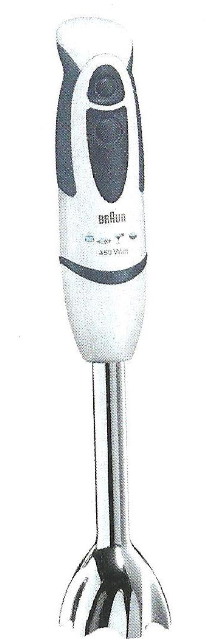
\includegraphics[width=1cm]{braum-mixer} % Reemplaza con tu imagen
        \caption*{Ganador del concurso de batidoras indesmontables... Braum y Kenwood!}
    \end{minipage}
    \hfill
    \begin{minipage}[b]{0.4\textwidth}
        \centering
        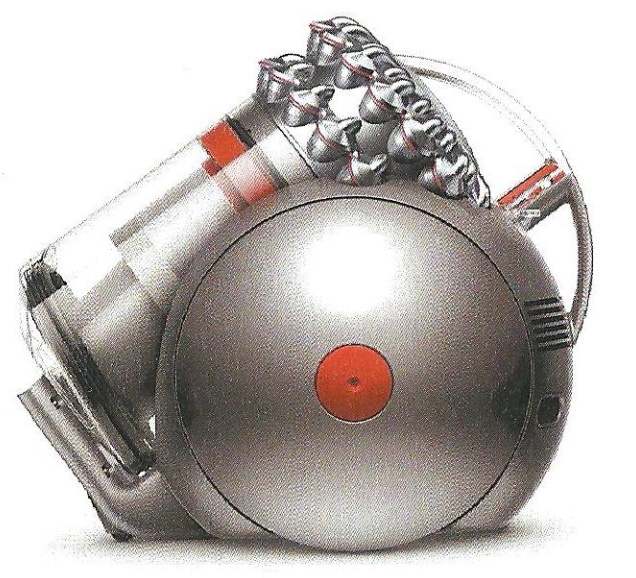
\includegraphics[width=2cm]{Dyson} % Reemplaza con tu imagen
        \caption*{¿Es para aspirar polvo intergaláctico?}
    \end{minipage}
\end{figure}



\end{itemize}


\chapter{Las bases de la electricidad}
\section{¿Qué es la electricidad?}
Con un poco de teoría, voy a explicar algunos conceptos básicos
para que entiendas lo que es la electricidad.
Así podrás medir y probar muchos de los componentes de tus
en tus electrodomésticos.

\begin{figure}[h]
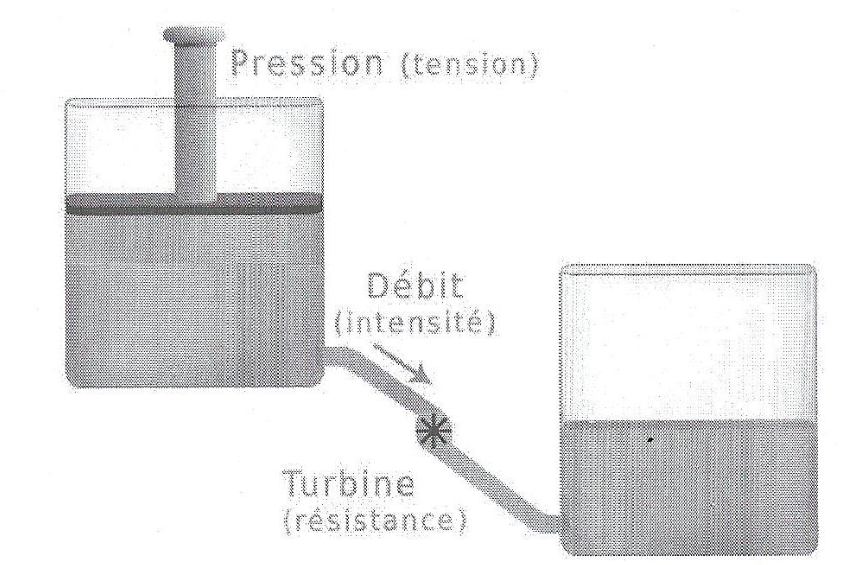
\includegraphics[width=0.8\textwidth]{analogia-agua-elec} % Reemplaza con tu imagen
\caption*{Analogía entre la electricidad y el agua}
\end{figure}

\begin{itemize}
\item \textbf{La tensión (U)} se expresa en voltios (V). Puede ser \textbf{Contínua}, como en una batería, salida del cargador, etc.) o \textbf{Alterna} (señales de la red eléctrica
señales electrónicas, etc.). Es una diferencia de potencial eléctrico entre dos
dos puntos. Siempre medimos una tensión entre dos puntos. Veremos más tarde cómo hacerlo. La tensión de una batería puede ser de 1.5V, 3V, 9V, la tensión de red ronda actualmente los 230V.

\item \textbf{La intensidad (I)} (o "corriente") se expresa en amperios (A).
Flujo de electrones a través de un hilo conductor con una determinada impresión.
A diferencia de la tensión, para que exista una corriente debe consumirse energía.
debe consumirse energía. ë
No hay corriente medible en una pila que no está conectada a nada.
- En este caso, decimos que no tiene "carga" (lo que no significa que no esté cargada en el sentido de que no esté conectada a nada).
 que no esté cargada en el sentido de una pila descargada, significa que
que no está suministrando energía).

\item \textbf{La resistencia (R)} se expresa en ohmios $\Omega$. Es muy baja
(a menudo se considera nula) para los metales y muy alta para el aire
el aire, el plástico o la madera seca, por ejemplo.
Por tanto, un cable eléctrico tendrá una resistencia muy cercana a 0$\Omega$ y el aire tendrá
una resistencia considerada infinita.
Algunos componentes electrónicos o elementos eléctricos también se denominan "resistencias"
o elementos eléctricos (por ejemplo, la resistencia de un horno eléctrico
horno o tostadora).
También existen resistencias "variables", ya sea por acción mecánica o por un cambio de temperatura.
o por un cambio de temperatura, por ejemplo.

\end{itemize}

\noindent\fbox{%
    \parbox{\textwidth}{%
La relación entre estos tres valores es $U(V) = R(\Omega) \times I(A)$, lo que implica que para una tensión fija, si disminuye la resistencia, la intensidad aumenta, y vice versa. Esto se comprende bien gracias al esquema de analogía entre el agua y la electricidad!
    }%
}\\

Para medir estos tres valores eléctricos, necesitamos una herramienta especial llamada "multímetro". (véase el capítulo 2.4).

\begin{figure}[h]
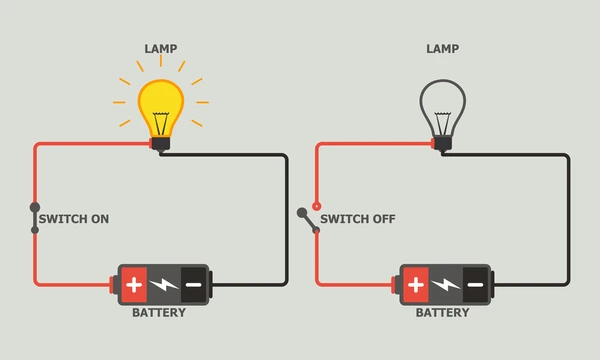
\includegraphics[width=0.7\textwidth]{circuito-abierto-cerrado} % Reemplaza con tu imagen
\centering
\caption*{Circuito abierto o cerrado (cambiar por otra figura)}
\end{figure}

\begin{enumerate}
\item Interruptor cerrado: la tensión "U" es igual a la tensión del generador, y ésta se extiende hasta los contactos de la lámpara (la tension en los extemos de un cable o de un interruptor cerrado siempre es de 0V). La corriente (I) existe y proporciona corriente a la lámpara para encenderse.
\item Interruptor abierto: la tensión "U" es igual a la tensión del generador, La tensión en los contactos de la lámpara es de 0V, no circula corriente
\end{enumerate}
La analogía con el agua no funciona aquí: un circuito cerrado significa que la electricidad puede circular.
posible circulación de electricidad, mientras que un grifo cerrado significa que no hay
circulación de agua...La analogía con el agua no funciona aquí: un circuito cerrado significa que la electricidad puede circular.
posible circulación de electricidad, mientras que un grifo cerrado significa que no hay
circulación de agua...

% Additional chapters...

\end{document}
